\documentclass[11pt,oneside]{article}
\usepackage[T1]{fontenc}
\usepackage[utf8]{inputenc}
% \usepackage{lmodern}
%\usepackage[adobe-utopia,uppercase=upright,greeklowercase=upright]{mathdesign}
\usepackage[adobe-utopia]{mathdesign}
%\usepackage{minionpro}
% \usepackage{pifont}
% \usepackage{amssymb}
\usepackage{amsmath}
\usepackage[francais]{babel}
% \usepackage[francais]{varioref}
\usepackage[dvips]{graphicx}

\usepackage{framed}
\usepackage[normalem]{ulem}
\usepackage{fancyhdr}
\usepackage{titlesec}
\usepackage{vmargin}
\usepackage{longtable}

\usepackage{ifthen}


%\usepackage{epsfig}
\usepackage{subfig}

\usepackage{multirow}
\usepackage{multicol} % Portions de texte en colonnes
\usepackage{flafter}%floatants après la référence



\usepackage{color}
\usepackage{colortbl}


\definecolor{gris25}{gray}{0.75}
\definecolor{bleu}{RGB}{18,33,98}
\definecolor{bleuf}{RGB}{42,94,171}
\definecolor{bleuc}{RGB}{231,239,247}
\definecolor{rougef}{RGB}{185,18,27}
\definecolor{rougec}{RGB}{255,230,231}
\definecolor{vertf}{RGB}{103,126,82}
\definecolor{vertc}{RGB}{220,255,191}

\newenvironment{rem}[1][\hsize]%
{%
    \def\FrameCommand
    {%
\rotatebox{90}{\textit{\textsf{Remarque}}} 
        {\color{bleuf}\vrule width 3pt}%
        \hspace{0pt}%must no space.
        \fboxsep=\FrameSep\colorbox{bleuc}%
    }%
    \MakeFramed{\hsize#1\advance\hsize-\width\FrameRestore}%
}%
{\endMakeFramed}%


\newenvironment{contexte}[1][\hsize]%
{%
    \def\FrameCommand
    {%
\rotatebox{90}{\textit{\textsf{Contexte}}} 
        {\color{bleuf}\vrule width 3pt}%
        \hspace{0pt}%must no space.
        \fboxsep=\FrameSep\colorbox{bleuc}%
    }%
    \MakeFramed{\hsize#1\advance\hsize-\width\FrameRestore}%
}%
{\endMakeFramed}%

\newenvironment{savoir}[1][\hsize]%
{%
    \def\FrameCommand
    {%
\rotatebox{90}{\textit{\textsf{Savoir}}} 
        {\color{bleuf}\vrule width 3pt}%
        \hspace{0pt}%must no space.
        \fboxsep=\FrameSep\colorbox{bleuc}%
    }%
    \MakeFramed{\hsize#1\advance\hsize-\width\FrameRestore}%
}%
{\endMakeFramed}%

\newenvironment{prob}[1][\hsize]%
{%
    \def\FrameCommand%
    {%
\rotatebox{90}{\textit{\textsf{ Problématique}}} 
        {\color{rougef}\vrule width 3pt}%
        \hspace{0pt}%must no space.
        \fboxsep=\FrameSep\colorbox{rougec}%
    }%
    \MakeFramed{\hsize#1\advance\hsize-\width\FrameRestore}%
}%
{\endMakeFramed}%

\newenvironment{obj}[1][\hsize]%
{%
    \def\FrameCommand%
    {%
\rotatebox{90}{\textit{\textsf{ $\;$}}} 
        {\color{rougef}\vrule width 3pt}%
        \hspace{0pt}%must no space.
        \fboxsep=\FrameSep\colorbox{rougec}%
    }%
    \MakeFramed{\hsize#1\advance\hsize-\width\FrameRestore}%
}%
{\endMakeFramed}%

\newenvironment{defi}[1][\hsize]%
{%
    \def\FrameCommand%
    {%
\rotatebox{90}{\textit{\textsf{Définition\\}}} 
        {\color{bleuf}\vrule width 3pt}%
        \hspace{0pt}%must no space.
        \fboxsep=\FrameSep\colorbox{bleuc}%
    }%
    \MakeFramed{\hsize#1\advance\hsize-\width\FrameRestore}%
}%
{\endMakeFramed}%


\newenvironment{hypo}[1][\hsize]%
{%
    \def\FrameCommand%
    {%
\rotatebox{90}{\textit{\textsf{Hypothèse\\}}} 
        {\color{bleuf}\vrule width 3pt}%
        \hspace{0pt}%must no space.
        \fboxsep=\FrameSep\colorbox{bleuc}%
    }%
    \MakeFramed{\hsize#1\advance\hsize-\width\FrameRestore}%
}%
{\endMakeFramed}%


\newenvironment{prop}[1][\hsize]%
{%
    \def\FrameCommand%
    {%
\rotatebox{90}{\textit{\textsf{Propriété\\}}} 
        {\color{bleuf}\vrule width 3pt}%
        \hspace{0pt}%must no space.
        \fboxsep=\FrameSep\colorbox{bleuc}%
    }%
    \MakeFramed{\hsize#1\advance\hsize-\width\FrameRestore}%
}%
{\endMakeFramed}%

\newenvironment{props}[1][\hsize]%
{%
    \def\FrameCommand%
    {%
\rotatebox{90}{\textit{\textsf{Propriétés\\}}} 
        {\color{bleuf}\vrule width 3pt}%
        \hspace{0pt}%must no space.
        \fboxsep=\FrameSep\colorbox{bleuc}%
    }%
    \MakeFramed{\hsize#1\advance\hsize-\width\FrameRestore}%
}%
{\endMakeFramed}%

\newenvironment{exemple}[1][\hsize]%
{%
    \def\FrameCommand%
    {%
\rotatebox{90}{\textit{\textsf{Exemple\\}}} 
        {\color{vertf}\vrule width 3pt}%
        \hspace{0pt}%must no space.
        \fboxsep=\FrameSep\colorbox{vertc}%
    }%
    \MakeFramed{\hsize#1\advance\hsize-\width\FrameRestore}%
}%
{\endMakeFramed}%

\newenvironment{resultat}[1][\hsize]%
{%
    \def\FrameCommand%
    {%
\rotatebox{90}{\textit{\textsf{Résultat\\}}} 
        {\color{rougef}\vrule width 3pt}%
        \hspace{0pt}%must no space.
        \fboxsep=\FrameSep\colorbox{rougec}%
    }%
    \MakeFramed{\hsize#1\advance\hsize-\width\FrameRestore}%
}%
{\endMakeFramed}%

\newenvironment{methode}[1][\hsize]%
{%
    \def\FrameCommand%
    {%
\rotatebox{90}{\textit{\textsf{Méthode\\}}} 
        {\color{rougef}\vrule width 3pt}%
        \hspace{0pt}%must no space.
        \fboxsep=\FrameSep\colorbox{rougec}%
    }%
    \MakeFramed{\hsize#1\advance\hsize-\width\FrameRestore}%
}%
{\endMakeFramed}%

\newenvironment{theo}[1][\hsize]%
{%
    \def\FrameCommand%
    {%
\rotatebox{90}{\textit{\textsf{Théorème\\}}} 
        {\color{rougef}\vrule width 3pt}%
        \hspace{0pt}%must no space.
        \fboxsep=\FrameSep\colorbox{rougec}%
    }%
    \MakeFramed{\hsize#1\advance\hsize-\width\FrameRestore}%
}%
{\endMakeFramed}%

\newenvironment{warn}[1][\hsize]%
{%
    \def\FrameCommand%
    {%
\rotatebox{90}{\textit{\textsf{Attention\\}}} 
        {\color{rougef}\vrule width 3pt}%
        \hspace{0pt}%must no space.
        \fboxsep=\FrameSep\colorbox{rougec}%
    }%
    \MakeFramed{\hsize#1\advance\hsize-\width\FrameRestore}%
}%
{\endMakeFramed}%

% \usepackage{pstricks}
%\usepackage{minitoc}
% \setcounter{minitocdepth}{4}

\setcounter{tocdepth}{2}

% \mtcselectlanguage{french} 

%\usepackage{draftcopy}% "Brouillon"
% \usepackage{floatflt}
\usepackage{psfrag}
%\usepackage{listings} % Permet d'insérer du code de programmation
\renewcommand{\baselinestretch}{1.2}

% Changer la numérotation des figures :
% ------------------------------------
% \makeatletter
% \renewcommand{\thefigure}{\ifnum \c@section>\z@ \thesection.\fi
%  \@arabic\c@figure}
% \@addtoreset{figure}{section}
% \makeatother
 


%%%%%%%%%%%%
% Définition des vecteurs %
%%%%%%%%%%%%
 \newcommand{\vect}[1]{\overrightarrow{#1}}

%%%%%%%%%%%%
% Définition des torseusr %
%%%%%%%%%%%%

 \newcommand{\torseur}[1]{%
\left\{{#1}\right\}
}

\newcommand{\torseurcin}[3]{%
\left\{\mathcal{#1} \left(#2/#3 \right) \right\}
}

\newcommand{\torseurstat}[3]{%
\left\{\mathcal{#1} \left(#2\rightarrow #3 \right) \right\}
}

 \newcommand{\torseurc}[8]{%
%\left\{#1 \right\}=
\left\{
{#1}
\right\}
 = 
\left\{%
\begin{array}{cc}%
{#2} & {#5}\\%
{#3} & {#6}\\%
{#4} & {#7}\\%
\end{array}%
\right\}_{#8}%
}

 \newcommand{\torseurcol}[7]{
\left\{%
\begin{array}{cc}%
{#1} & {#4}\\%
{#2} & {#5}\\%
{#3} & {#6}\\%
\end{array}%
\right\}_{#7}%
}

 \newcommand{\torseurl}[3]{%
%\left\{\mathcal{#1}\right\}_{#2}=%
\left\{%
\begin{array}{l}%
{#1} \\%
{#2} %
\end{array}%
\right\}_{#3}%
}

 \newcommand{\vectv}[3]{%
\vect{V\left( {#1} \in {#2}/{#3}\right)}
}


\newcommand{\vectf}[2]{%
\vect{R\left( {#1} \rightarrow {#2}\right)}
}

\newcommand{\vectm}[3]{%
\vect{\mathcal{M}\left( {#1}, {#2} \rightarrow {#3}\right)}
}


 \newcommand{\vectg}[3]{%
\vect{\Gamma \left( {#1} \in {#2}/{#3}\right)}
}

 \newcommand{\vecto}[2]{%
\vect{\Omega\left( {#1}/{#2}\right)}
}
% }$$\left\{\mathcal{#1} \right\}_{#2} =%
% \left\{%
% \begin{array}{c}%
%  #3 \\%
%  #4 %
% \end{array}%
% \right\}_{#5}}

%  ------------------------------------------
% | Modification du formatage des sections : | 
%  ------------------------------------------

% Grands titres :
% ---------------

\newcommand{\titre}[1]{%
\begin{center}
      \bigskip
      \rule{\textwidth}{1pt}
      \par\vspace{0.1cm}
      
      \textbf{\large #1}
      \par\rule{\textwidth}{1pt}
    \end{center}
    \bigskip
  }

% Supprime le numéro du chapitre dans la numérotation des sections:
% -----------------------------------------------------------------
\makeatletter
\renewcommand{\thesection}{\@arabic\c@section}
\makeatother


% \titleformat{\chapter}[display]
% {\normalfont\Large\filcenter}
% {}
% {1pc}
% {\titlerule[1pt]
%   \vspace{1pc}%
%   \Huge}[\vspace{1ex}%
% \titlerule]


%%%% Chapitres Comme PY Pechard %%%%%%%%%
% numéro du chapitre
\DeclareFixedFont{\chapnumfont}{OT1}{phv}{b}{n}{80pt}
% pour le mot « Chapitre »
\DeclareFixedFont{\chapchapfont}{OT1}{phv}{m}{it}{40pt}
% pour le titre
\DeclareFixedFont{\chaptitfont}{T1}{phv}{b}{n}{25pt}

\definecolor{gris}{gray}{0.75}
\titleformat{\chapter}[display]%
	{\sffamily}%
	{\filleft\chapchapfont\color{gris}\chaptertitlename\
	\\
	\vspace{12pt}
	\chapnumfont\thechapter}%
	{16pt}%
	{\filleft\chaptitfont}%
	[\vspace{6pt}\titlerule\titlerule\titlerule]

%%%%  Fin Chapitres Comme PY Pechard %%%%%%%%%


% Section, subsection, subsubsection sans serifs :
% % ----------------------------------------------

% \makeatletter
% \renewcommand{\section}{\@startsection{section}{0}{0mm}%
% {\baselineskip}{.3\baselineskip}%
% {\normalfont\sffamily\Large\textbf}}%
% \makeatother

\makeatletter
\renewcommand{\@seccntformat}[1]{{\textcolor{bleu}{\csname
the#1\endcsname}\hspace{0.5em}}}
\makeatother

\makeatletter
\renewcommand{\section}{\@startsection{section}{1}{\z@}%
                       {-4ex \@plus -1ex \@minus -.4ex}%
                       {1ex \@plus.2ex }%
                       {\normalfont\Large\sffamily\bfseries}}%
\makeatother
 
\makeatletter
\renewcommand{\subsection}{\@startsection {subsection}{2}{\z@}
                          {-3ex \@plus -0.1ex \@minus -.4ex}%
                          {0.5ex \@plus.2ex }%
                          {\normalfont\large\sffamily\bfseries}}
\makeatother
 
\makeatletter
\renewcommand{\subsubsection}{\@startsection {subsubsection}{3}{\z@}
                          {-2ex \@plus -0.1ex \@minus -.2ex}%
                          {0.2ex \@plus.2ex }%
                          {\normalfont\large\sffamily\bfseries}}
\makeatother
 
\makeatletter             
\renewcommand{\paragraph}{\@startsection{paragraph}{4}{\z@}%
                                    {-2ex \@plus-.2ex \@minus .2ex}%
                                    {0.1ex}%               
{\normalfont\sffamily\bfseries}}
\makeatother
 
\makeatletter             
\renewcommand{\paragraph}{\@startsection{paragraph}{4}{\z@}%
                                    {-2ex \@plus-.2ex \@minus .2ex}%
                                    {0.1ex}%               
{\normalfont\sffamily\bfseries Question }}
\makeatother

\renewcommand{\theparagraph}{\arabic{paragraph}} 


\makeatletter
\renewcommand{\subparagraph}{\@startsection{subparagraph}{5}{\z@}%
                                       {-2ex \@plus-.1ex \@minus .2ex}%
                                       {0.1ex}%
				    {\normalfont\normalsize\sffamily\bfseries}}
\makeatletter
% \makeatletter
% \renewcommand{\subsection}{\@startsection{subsection}{1}{2mm}%
% {\baselineskip}{.3\baselineskip}%
% {\normalfont\sffamily\large\textbf}}%
% \makeatother
% 
% \makeatletter
% \renewcommand{\subsubsection}{\@startsection{subsubsection}{2}{4mm}%
% {\baselineskip}{.15\baselineskip}%
% {\normalfont\sffamily\large\textbf}}%
% \makeatother
% 
% \makeatletter
% \renewcommand{\paragraph}{\@startsection{paragraph}{3}{6mm}%
% {\baselineskip}{.15\baselineskip}%
% {\normalfont\sffamily\large\textbf}}%
% \makeatother
 
\setcounter{secnumdepth}{4}


%  --------
% | Marges |
%  --------


% \setmarginsrb{2.5cm}{1.5cm}{2.5cm}{2cm}{1cm}{1cm}{1cm}{1cm}
\setmarginsrb{1.5cm}{1cm}{1cm}{1.5cm}{1cm}{1cm}{1cm}{1cm}

% Changer les marges localement :
% -----------------------------
\newenvironment{changemargin}[2]{\begin{list}{}{%
\setlength{\topsep}{0pt}%
\setlength{\leftmargin}{0pt}%
\setlength{\rightmargin}{0pt}%
\setlength{\listparindent}{\parindent}%
\setlength{\itemindent}{\parindent}%
\setlength{\parsep}{0pt plus 1pt}%
\addtolength{\leftmargin}{#1}%
\addtolength{\rightmargin}{#2}%
}\item }{\end{list}}



\usepackage{pst-solides3d}
\usepackage{titletoc}
\titlecontents{chapter}[+3pc]
  {\addvspace{10pt}\sffamily\bfseries}
{\contentslabel[{\pscirclebox[fillstyle=solid,fillcolor=gray!25,
linecolor=gray!25,framesep=4pt]{\textcolor{white}{\thecontentslabel}}}]{2.5pc}}
  {}
  {\dotfill \normalfont\thecontentspage\ }

\titlecontents{section}[3pc]
  {\addvspace{2pt}\sffamily}
  {\contentslabel[\thecontentslabel]{1.8pc}}
  {}
  {\dotfill \normalfont\thecontentspage\ }

\titlecontents{subsection}[5pc]
  {\addvspace{2pt}\sffamily}
  {\contentslabel[\thecontentslabel]{1.8pc}}
  {}
  {\dotfill \normalfont\thecontentspage\ }

\titlecontents{subsubsection}[8pc]
  {\addvspace{2pt}\sffamily}
  {\contentslabel[\thecontentslabel]{3pc}}
  {}
  {\dotfill \normalfont\thecontentspage\ }
%{\;\titlerule\;\normalfont\thecontentspage\ }

\titlecontents{paragraph}[9pc]
  {\addvspace{2pt}\sffamily}
  {\contentslabel[\thecontentslabel]{3.5pc}}
  {}
  {\dotfill \normalfont\thecontentspage\ }




\usepackage[%
    pdftitle={Cinématique - DM5},
    pdfauthor={Xavier Pessoles},
    colorlinks=true,
    linkcolor=blue,
    citecolor=magenta]{hyperref}

\usepackage{schemabloc}

% \makeatletter \let\ps@plain\ps@empty \makeatother
%% DEBUT DU DOCUMENT
%% =================
\sloppy
\hyphenpenalty 10000

\newcommand{\Pointilles}[1][3]{%
\multido{}{#1}{\makebox[\linewidth]{\dotfill}\\[\parskip]
}}


\colorlet{shadecolor}{orange!15}

\newtheorem{theorem}{Theorem}

\newenvironment{theo}
  {\begin{snugshade}\begin{leftbar}\begin{theorem}}
  {\end{theorem}\end{leftbar}\end{snugshade}}


\renewenvironment{leftbar}[1][\hsize]
{%
    \def\FrameCommand
    {%
        {\color{bleuf}\vrule width 3pt}%
        \hspace{0pt}%must no space.
        \fboxsep=\FrameSep\colorbox{bleuc}%
    }%
    \MakeFramed{\hsize#1\advance\hsize-\width\FrameRestore}%
}
{\endMakeFramed}




\begin{document}


\newboolean{prof}
\setboolean{prof}{true}
%------------- En tetes et Pieds de Pages ------------
\pagestyle{fancy}
\renewcommand{\headrulewidth}{0pt}

\fancyhead{}
\fancyhead[L]{%
\begin{minipage}[c]{1.6cm}

\includegraphics[width=1.4cm]{png/logo_jh_ptsi.png}%
\end{minipage}
\rule{2cm}{.5pt}
}

\fancyhead[C]{\rule{12cm}{.5pt}}

\fancyhead[R]{%
\begin{minipage}[c]{3cm}
\begin{flushright}
\footnotesize{\textit{\textsf{Sciences Industrielles\\ pour l'Ingénieur}}}%
\end{flushright}
\end{minipage}
}

\renewcommand{\footrulewidth}{0.2pt}

\fancyfoot[C]{\footnotesize{\bfseries \thepage}}
\fancyfoot[L]{\footnotesize{2011 -- 2012} \\ X. \textsc{Pessoles}}
\ifthenelse{\boolean{prof}}{%
\fancyfoot[R]{\footnotesize{DM 5 -- CI 2 : SLCI -- P}}
}{%
\fancyfoot[R]{\footnotesize{DM 5 -- CI 2 : SLCI}}
}


%\begin{center}
%\textit{Centre d'intérêt}
%\end{center}

\begin{center}
 \Large\textsc{Devoir Maison 5}
\end{center}

\begin{center}
 \large\textsc{A rendre le mercredi 4 janvier} 
\end{center}

\vspace{.25cm}

\begin{center}
 \large\textsc{} 
\end{center}

\vspace{.25cm}

\section{Mise en situation}

Pour offrir une prestation internationale complète, la branche fret de la SNCF développe de plus en plus le transport combiné associant le mode ferroviaire aux autres modes de transport : route, maritime ou fluvial. L'objectif est de transférer directement sur des wagons les conteneurs portés par les camions, les navires ou  les péniches.

Pour assurer une meilleure maîtrise de la continuité du transport, la tendance actuelle est de faire circuler à des vitesses de plus en plus élevées des wagons de marchandises susceptibles de recevoir des charges de plus en plus importantes par rapport au poids à vide du wagon.
Pour obtenir une grande puissance de freinage sans risque quel que soit l'état de charge des wagons de fret, la société SAB WABCO a mis au point un dispositif de freinage qui équipe les wagons de fret de la SNCF.

\subsection{Description du dispositif}
\begin{minipage}[c]{.3\linewidth}
C'est un système entièrement mécanique : ce mécanisme est volontairement dépourvu d'électronique afin d'augmenter sa fiabilité. Il permet d'obtenir une puissance de freinage proportionnelle à la charge du wagon et est composé de 2 modules : 
\begin{itemize}
\item un module d'amplification qui sert à la production et à l'amplification de l'effort de freinage.
\item un module de pesée qui permet de modifier l'effort de freinage en fonction de la charge du wagon.
\end{itemize}
\end{minipage}
\hfill
\begin{minipage}[c]{.65\linewidth}
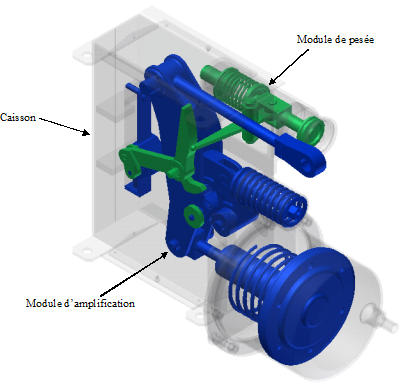
\includegraphics[width=.95\textwidth]{png/img1}
\end{minipage}

\subsection*{Le module de pesée}
(Ce module ne sera pas étudié ici)

Un détendeur de pesée placé sous le wagon détermine sa charge et délivre à sa sortie une pression d'air proportionnelle à la charge du wagon. Cette pression permet par l'intermédiaire d'un piston et d'un levier de modifier la position verticale de la butée mobile 26.

\subsection*{Le module d'amplification}
Alimenté par une pression constante de 4 bars, le piston du cylindre de frein pousse, par le biais de la tige 28, le balancier 21 qui prend appui sur la butée mobile 26. Le balancier 21, suspendu au bras 27 et en appui sur la butée 26, transmet un effort adapté (multiplié ou réduit selon la charge du wagon) à la bielle de poussée 19. Cet effort est transmis par une timonerie aux sabots de frein et sert au freinage effectif du wagon.
\subsection{Fonctionnement}
On ne s'intéresse ici qu'au module d'amplification.
L'activation du cycle de freinage se décompose en 3 phases :

\begin{center}
\begin{tabular}{|p{.3\textwidth}|p{.3\textwidth}|p{.3\textwidth}|}
\hline 
Phase 1 : approche rapide des sabots de freins &
Phase 2 : accostage du balancier 21 sur la butée mobile 26 & 
Phase 3 : freinage effectif \\
\hline
\begin{center}
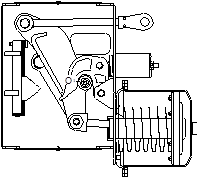
\includegraphics[width=.3\textwidth]{png/img2}
\end{center}&
\begin{center}
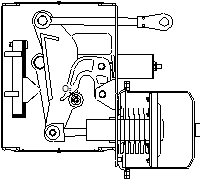
\includegraphics[width=.3\textwidth]{png/img3}
\end{center}&
\begin{center}
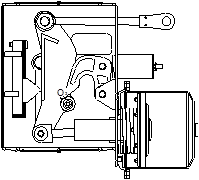
\includegraphics[width=.3\textwidth]{png/img4} 
\end{center}\\
\hline
Le galet 37 est en contact (point O1) avec la zone 1 du crochet guide 20. Le plan de ce contact étant pratiquement vertical, le basculement du balancier 21 est alors très rapide.&
Durant cette phase, le balancier 21 bascule autour de l'axe 22 pour venir en contact avec la butée 
mobile 26, avec un mouvement d'approche plus lent que le précédent.

Le galet 37 est en contact (point O2) avec la zone 2 du crochet guide 20.&

	Le balancier 21 est maintenant en contact avec la butée mobile 26. 
La butée mobile 26 sert d'appui au balancier 21  pour faire varier l'effort de freinage.
Le galet 37 est en contact (point O3) avec la zone 3 du crochet guide 20. \\
\hline
\end{tabular}
\end{center}
	
 
 \section{Travail demandé}
	
 
Afin de pouvoir identifier rapidement les problèmes en cas d'incident, le constructeur désire que la phase d'approche des sabots de frein vers les roues du wagon (phase 1) et la phase d'accostage du balancier 21 vers la butée mobile 26 (phase 2) soient pratiquement indépendantes l'une de l'autre. Pour cela, l'axe 22 doit se déplacer rapidement pendant la phase 1 pour une approche rapide des sabots de frein puis doit progressivement s'immobiliser au cours de la phase 2 (approche lente) pour permettre un accostage correct entre le balancier 21 et la butée mobile 26.
Afin de vérifier ces faits qui font partie du cahier des charges fonctionnel, on se propose d'effectuer la modélisation cinématique qui permettra de mettre en équation les paramètres cinématiques du mouvement de ce mécanisme.
 
Le plan d'ensemble, la nomenclature et la vue en perspective vous permettront de repérer toutes les pièces.
\subsection*{Hypothèses et données}
\begin{itemize}
\item on s'intéresse au mécanisme en phase 1 ou 2, lorsqu'il n'y a pas encore contact de 27 sur la butée 26. Les pièces 26, 25, 24 seront donc considérées comme encastrées avec le bâti;
\item les pièces 45 et 10 sont soudées entre elles;
\item l'indication en coupe B-B donnant « 20H7g6 » indique que les pièces 30 et 27 sont montées glissantes : il existe en effet un petit jeu entre l'arbre 30 et l'alésage de 27 qui fait que ces deux pièces ne sont pas serrées l'une dans l'autre (la rotation / axe de révolution est alors possible).
Il en est de même pour : 28/46 ; 28/41 ; 21/41;
\item les pièces 47 et 3 sont montées glissantes également;
\item les couples de pièces suivantes sont frettées entre elles : \{45+47\};\{axeC+21\};\{22+19\};\{46+45\};
\item les pièces 40+39+27 sont encastrées entre elles, et la bague 38 est serrée dans le galet 37.
\end{itemize}

\subsection{Questions préliminaires}
\paragraph{}
\textit{Rechercher et expliquer ce que signifie le terme « pièces frettées ».}

%\paragraph{}
%\textit{Quel est le rôle de la pièce 38 ?}

\paragraph{}
\textit{Quels sont le nom et le rôle de la pièce 29 ?}

\paragraph{}
\textit{Quel est le rôle, dans le fonctionnement de ce mécanisme, du ressort 5 ?}

\paragraph{}
\textit{Quel est le rôle du ressort 16 ?}

\paragraph{}
\textit{Rechercher ce que signifie précisément les désignations de matériaux donnés dans la nomenclature pour les pièces 5, 10, 38. Pour la pièce 10, vous expliciterez comment est déterminée la valeur 295. }

\paragraph{}
\textit{Donner l'ensemble des opérations qui ont mené à la fabrication des pièces 1, 3, 27 et 39. (En partant d'un lopin ou d'un lingot de métal, en arrivant à la forme finie.)}



\subsection{Modélisation cinématique}
\paragraph{}
\textit{Déterminer les classes d'équivalence de ce mécanisme : pour ce faire, associer une couleur à chaque groupe défini, et « colorier » la vue de face en coupe A-A ainsi que les coupes B-B, C-C et D-D du plan d'ensemble. Faire également la liste des pièces par groupe et donner un nom a chaque groupe (utiliser le repère de la pièce principal du groupe).}

\paragraph{}
\textit{Identifier les liaisons entre ces classes. Vous préciserez obligatoirement la nature des surfaces en contact, justifiant ainsi les liaisons déterminées. Donner le schéma plan et 3D des liaisons en respectant les couleurs choisies pour les classes d'équivalence de la question précédente. Le repère doit être identique pour tous les schémas.}
			
\paragraph{}
\textit{Effectuer le schéma cinématique plan de ce mécanisme, en couleurs (identiques aux classes d'équivalence) dans le plan de la coupe A-A, et à l'échelle du plan fourni.
 Utilisez  le plan pour positionner les centres et les axes des liaisons 
 Vous respecterez les solutions constructives choisies pour le mécanisme concernant les pièces qui seront considérées comme « axe » ou comme « alésage » de la liaison.}


\paragraph{}
\textit{Effectuer un paramétrage pour chacun des types de liaisons. (Par exemple, s'il existe 3 pivots et 2 rotules dans le dessin, vous n'effectuerez qu'un seul paramétrage pour une des pivots et 1 paramétrage pour une des rotules.}


\paragraph{}
\textit{Effectuer ce schéma en perspective, en couleur.
 Son orientation est au choix.
 On ne demande pas de respecter l'échelle, mais vous devez respecter les positions relatives des liaisons}

\subsection{Étude technologique de certaines liaisons}

La liaison entre la tige de piston 28 et le piston 10 a fait l'objet de plusieurs évolutions technologiques. On se propose ici d'étudier pourquoi ces différentes solutions ont été abandonnées au profit de la solution actuelle représentée dans le plan d'ensemble
\subsection*{Analyse de la 1\iere solution (voir dessin ci-après)}

\paragraph{}
\textit{Préciser la nature de la liaison entre la tige de piston 28 et le piston 10 dans la solution 1 présentée ci-dessous et décrire sa réalisation technologique.}
\paragraph{}
\textit{A votre avis, quelle conséquence technique peut avoir le léger débattement angulaire de la tige 28 sur cette solution ? Justifier ainsi l'abandon de cette solution.}

\subsection*{Analyse de la 2\ieme solution}

\paragraph{}
\textit{Préciser la nature de la liaison entre la tige de piston 28 et le piston 10 dans cette solution 2.}

\paragraph{}
\textit{Cette liaison résout-elle le problème du débattement angulaire mis en évidence dans la 1ere solution ? Justifier votre réponse.}

      \begin{center}
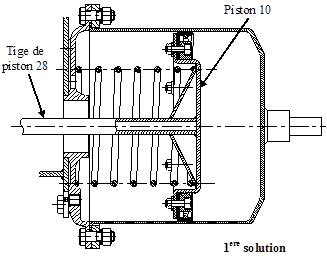
\includegraphics[width=.45\textwidth]{png/img5}
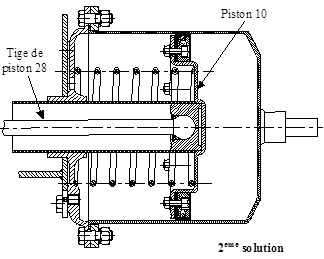
\includegraphics[width=.45\textwidth]{png/img6}
\end{center}

\paragraph{}
\textit{Quelle liaison a finalement été adoptée sur la solution finale, et quelle peut en être la raison.
Analyse de la liaison 47/3
Lors de la maintenance du mécanisme, on a pu remarquer une usure prématurée de l'alésage du flasque 3 au niveau du contact avec le tube 47.
On cherche à modéliser la liaison réalisée entre le tube 47 et le flasque 3, afin de pouvoir évaluer les actions mécaniques subies dans cette zone et éventuellement choisir une autre solution de conception.}

\paragraph{}
\textit{En considérant qu'il n'y a aucun jeu possible,  quel modèle peut on proposer pour cette liaison.}

\paragraph{}
\textit{Considérons maintenant qu'un léger jeu existe, impliquant un rotulage possible entre ces deux pièces, autour de deux axes supplémentaires. Quel modèle devrait-on alors adopter.}

\paragraph{}
\textit{L'usure observée au niveau de ce contact a tendance à augmenter ce jeu considérablement. Quelle solution simple pourriez vous proposer pour éviter cette usure.}
 

\vspace{2cm}

Le prof de SII m'a donné un DM pour le mercredi de la rentrée. Je l'ai pris... Je l'ai regardé... Je me suis demandé(e) pourquoi il met toujours un "I" après le "I" de "SI". J'ai réfléchi... J'ai soufflé... Je me suis dit que les vacances suffiraient bien à savoir pourquoi il y a deux I... Il y avait encore une histoire de train... ça changera des avions. Bref, je l'ai rangé. 

Les vacances ont commencé. Je suis allé(e) à la soif. Je suis rentré(e) tard... enfin tôt... enfin, je sais plus... Je me suis levé(e) pour aller en cours... En fait, les vacances n'avaient pas vraiment commencé. Je suis allé(e) en colle... J'aurais dû me laver les dents 2 fois.

J'ai pris le train, je suis rentré(e) chez moi. Je me suis dit tiens, je vais profiter du premier WE pour faire tous les DM histoire d'être tranquille. J'ai ouvert mon sac. **** m'a appelé(e). J'ai posé mon sac. **** a raccroché. Je me suis dis qu'elle (il) était quand même trop ****. J'ai repris mon sac. **** m'a appelé(e) pour aller au ciné. J'ai posé mon sac. Il (elle) a raccroché. J'ai repris mon sac. Je l'ai vidé dans un tiroir. Je suis parti au ciné.

Le lendemain matin, je me suis quand même dit que j'allais lire le DM de SII, peut être que le prof pas drôle aura mis une blague. J'ai ouvert le tiroir. Ma mère m'a appelé. J'ai fermé le tiroir. Je suis allé(e) ranger mon bol. Je suis remonté(e). J'ai ouvert le tiroir. Ma mère m'a appelé. J'ai fermé le tiroir. Je suis allé(e) essuyé la table. Je suis remonté(e). J'ai ouvert le tiroir. Mon frère jouait à la play. J'ai fermé le tiroir...

Mardi 3 janvier 21h00. 

Je suis retourné(e) à l'internat. Je me suis dis "Tiens, il y avait pas un DM de SI ?". Je me souvenais que ça parlait vaguement de train. Je suis allé sur google. J'ai tapé DM SI TRAIN. Je suis allé(e) sur le premier site. Rien. Je suis allé(e) sur le deuxième site. Rien. Je suis allé(e) sur le troisième. Rien. Je me suis dit que c'était peut être pour ça qu'il y a deux I à SII... J'ai réessayé... Rien... C'était quand même plus facile avec le Space Mountain... J'ai cherché le sujet dans mon sac... Rien. Je suis allé(e) dans la chambre d'à coté trouver un sujet. Ils avaient fini le DM (NDLR j'y crois pas). J'ai recopié le DM. J'ai ajouté des fautes. J'ai rangé le DM. 

Bref, j'ai fait le DM de SII des vacances de Noël. 

\section{Annexes}
\subsection{Vue en perspective du dispositif de freinage}
\begin{center}
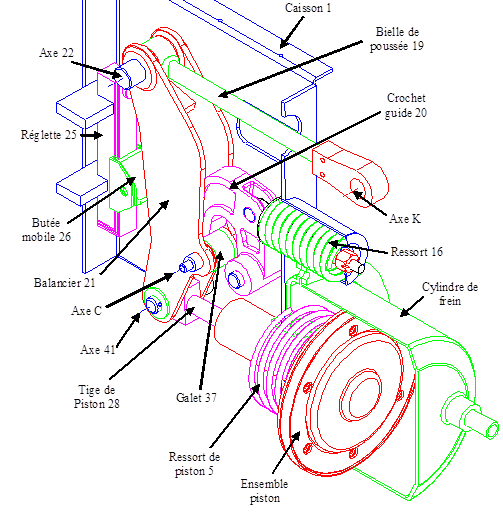
\includegraphics[width=.8\textwidth]{png/img7}
\end{center}

\subsection{Vue arrière, de détail et en perspective du bras 27}
\begin{center}
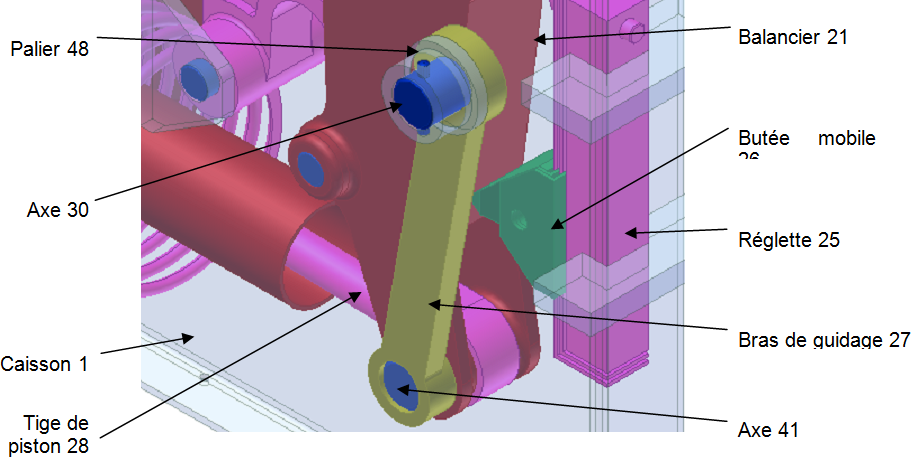
\includegraphics[width=.8\textwidth]{png/img8}
\end{center}

\subsection{Diagramme FAST du dispositif AC3}
\begin{center}
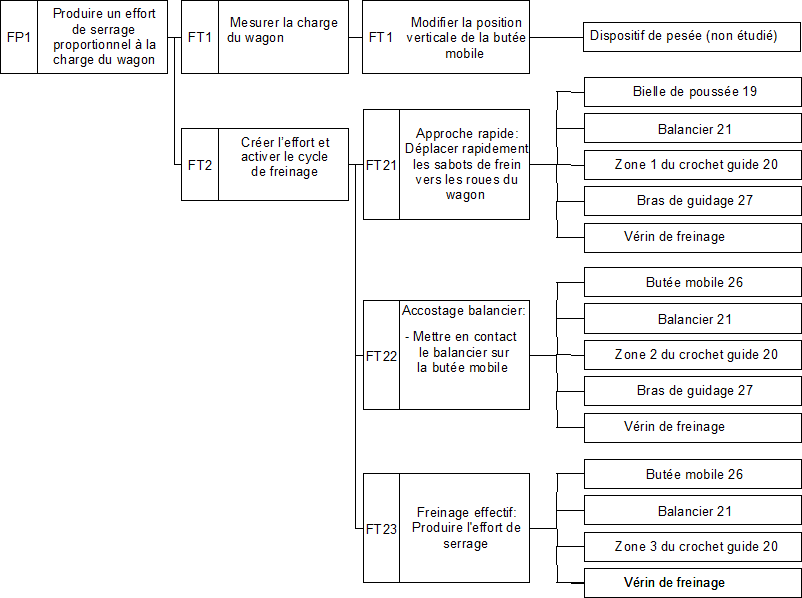
\includegraphics[width=.95\textwidth]{png/img9}
\end{center}


\subsection{Perspective éclatée du sous-ensemble piston}
\begin{center}
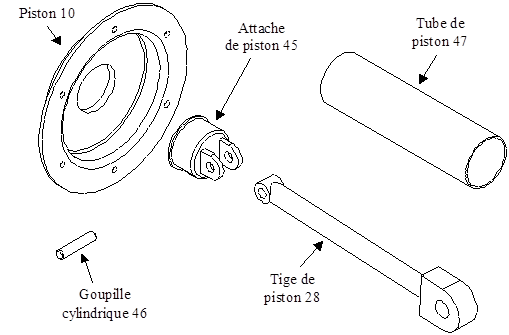
\includegraphics[width=.95\textwidth]{png/img10}
\end{center}

\subsection{Nomenclature}

\begin{center}
\rotatebox{90}{%
\footnotesize{%
\begin{tabular}{|l|l|l|l|l|}
\hline
Rep&	Nb&	Désignation&	Matière&	Observation \\
\hline
1&	1&	Caisson&	S 235&	\\\hline
2&	1&	Bouchon tête carrée&		&\\\hline
3&	1&	Flasque support &E 295&	\\\hline
4&	1&	Collier de fixation	&E 295&	\\\hline
5&	1&	Ressort de rappel du piston	&C 60&	\\\hline
6&	1&	Corps de cylindre	&E 295&	\\\hline
7&	1&	Cuir de piston		&&\\\hline
8&	1&	Jonc de garniture	&E 295&	\\\hline
9&	1&	Rondelle de piston	&E 295&	\\\hline
10&	1&	Piston	&E 295	&\\\hline
11&	1&	Manchon d’arrivée d’air&&		\\\hline
12&	1&	Rondelle d’appui		&&\\\hline
13&	1&	Goupille V 4 x 55	&	&NF E 27 - 487\\\hline
14&	1&	Douille filetée	&E 295&	\\\hline
15&	1&	Biellette du crochet guide	&E 295&	\\\hline
16&	1&	Ressort du crochet guide	&C 60	&\\\hline
17&	1&	Tenon de la bielle de poussée	&E 295&	\\\hline
18&	2&	Goupille cylindrique type A 8 x 40&		&NF E 27 - 484\\\hline
19&	1&	Bielle de poussée	&E 295&	\\\hline
20&	1&	Crochet guide	&E 295&	\\\hline
21&	1&	Balancier	&E 295&	\\\hline
22&	1&	Axe de bielle de poussée	&E 295&	\\\hline
23&	2&	Plaque de visite	&S 235&	\\\hline
24&	1&	Axe de retenue des lamelles guides	&E 295&	\\\hline
\end{tabular}
\begin{tabular}{|l|l|l|l|l|}
\hline
Rep&	Nb&	Désignation&	Matière&	Observation \\
\hline
25&	1&	Réglette	&E 295&	\\\hline
26&	1&	Butée mobile	&E 295&	\\\hline
27&	1&	Bras de guidage	&E 295&	\\\hline
28&	1&	Tige de piston	&E 295&	\\\hline
29&	1&	Goupille cannelée type G7 8 x 60&		&NF E 27 - 496\\\hline
30&	1&	Axe du bras de guidage	&E 295&	\\\hline
31&	1&	Lamelle guide intérieure	&S 235&	\\\hline
32&	1&	Lamelle guide extérieure	&S 235&	\\\hline
33&	1&	Axe de butée mobile	&E 295&	\\\hline
34&	1&	Plaque de frottement intérieur	&S 235&	\\\hline
35&	1&	Plaque de frottement extérieur	&S 235&	\\\hline
36&	1&	Goupille cylindrique type A 8 x 55&		&NF E 27 - 484\\\hline
37&	1&	Galet guide	&E 295&	\\\hline
38&	1&	Bague d’usure du galet guide	&Cu Sn 18 Pb 15&	\\\hline
39&	1&	Goupille V 6 x 55	&	&NF E 27 - 487\\\hline
40&	1&	Rondelle plate M 8	&	&NF E 25 - 514\\\hline
41&	1&	Axe de tige de piston	&E 295&	\\\hline
42&	1&	Axe de biellette du crochet guide&	E 295&	\\\hline
43&	1&	Axe du crochet guide	&E 295&	\\\hline
44&	1&	Goupille cylindrique type A 6 x 55&		&NF E 27 - 484\\\hline
45&	1&	Attache de piston	&E 295&\\\hline
46&	1&	Goupille cylindrique type A 16 x 65		&NF E 27 - 484&\\\hline
47&	1&	Tube de piston	&E 295&	\\\hline
48&	1&	Palier	&E 295& \\\hline
\end{tabular}}}
\end{center}

\end{document}